\documentclass[10pt,fleqn]{article}
%\usepackage{graphicx}


\setlength{\topmargin}{-.75in}
\addtolength{\textheight}{2.00in}
\setlength{\oddsidemargin}{.00in}
\addtolength{\textwidth}{.75in}

\title{Math 4610 Lecture Notes \\
            \ \\
       Homework Repository Structure and Permissions 
  \footnote{These notes are part of an Open Resource Educational project
            sponsored by Utah State University}}

\author{Joe Koebbe}

\nofiles

\pagestyle{empty}

\setlength{\parindent}{0in}

% new math commands


\setlength{\oddsidemargin}{-0.25in}
\setlength{\evensidemargin}{-0.25in}
\setlength{\textwidth}{6.75in}
\setlength{\headheight}{0.0in}
\setlength{\topmargin}{-0.25in}
\setlength{\textheight}{9.00in}

\makeindex

\usepackage{mathrsfs}

%\usepackage[pdftex]{graphicx}
\usepackage{epstopdf}

\newcounter{beans}

\newcommand{\ds}{\displaystyle}
\newcommand{\limit}[2]{\displaystyle\lim_{#1\to#2}}

\newcommand{\binomial}[2]{\ \left( \begin{array}{c}
                                  #1 \\
                                  #2
                                 \end{array}
                            \right) \
                         }
\newcommand{\ExampleRule}[2]
  {
  \noindent
  \rule{\linewidth}{1pt}
  \begin{example}
    #1
    \label{#2}
  \end{example}
  \rule{\linewidth}{1pt}
  \vskip0.125in
  }

\newcommand{\defbox}[1]
  {
   \ \\
   \noindent
   \setlength\fboxrule{1pt}
   \fbox{
        \begin{minipage}{6.5in}
          #1
        \end{minipage}
        }
   \ \\
  }
\newcommand{\verysmallworkbox}[1]
  {
   \ \\
   \noindent
   \setlength\fboxrule{1pt}
   \fbox{
        \begin{minipage}{6.5in}
           #1
           \ \\
           \vskip0.5in \ \\
           \ \\
        \end{minipage}
        }
   \ \\
  }
\newcommand{\smallworkbox}[1]
  {
   \ \\
   \noindent
   \setlength\fboxrule{1pt}
   \fbox{
        \begin{minipage}{6.5in}
           #1
           \ \\
           \vskip2.5in \ \\
           \ \\
        \end{minipage}
        }
   \ \\
  }
\newcommand{\halfworkbox}[1]
  {
   \ \\
   \noindent
   \setlength\fboxrule{1pt}
   \fbox{
        \begin{minipage}{6.5in}
           #1 \hfill
           \ \\
           \vskip3.25in \ \\
           \ \\
        \end{minipage}
        }
   \ \\
  }
\newcommand{\largeworkbox}[1]
  {
   \ \\
   \noindent
   \setlength\fboxrule{1pt}
   \fbox{
        \begin{minipage}{6.5in}
           #1
           \ \\
           \vskip7.5in \ \\
           \ \\
        \end{minipage}
        }
   \ \\
  }
\newcommand{\flexworkbox}[2]
  {
   \ \\
   \noindent
   \setlength\fboxrule{1pt}
   \fbox{
        \begin{minipage}{6.5in}
           #1
           \ \\

           \vskip#2 \ \\
           \ \\
        \end{minipage}
        }
   \ \\
  }


% symbols for sets of numbers

\newcommand{\natnumb}{$\cal N$}
\newcommand{\whonumb}{$\cal W$}
\newcommand{\intnumb}{$\cal Z$}
\newcommand{\ratnumb}{$\cal Q$}
\newcommand{\irrnumb}{$\cal I$}
\newcommand{\realnumb}{$\cal R$}
\newcommand{\cmplxnumb}{$\cal C$}

% misc. commands

\newcommand{\mma}{{\it Mathematica}}
\newcommand{\sech}{\mbox{ sech}}
 
\newtheorem{theorem}{Theorem}
\newtheorem{example}{Example}
\newtheorem{definition}{Definition}
\newtheorem{problem}{Problem}

\setcounter{secnumdepth}{2}
\setcounter{tocdepth}{4}


\begin{document}
\maketitle
\newpage
%%%%%%%%%%%%%%%%%%%%%%%%%%%%%%%%%%%%%%%%%%%%%%%%%%%%%%%%%%%%%%%%%%%%%%%%%%%%%%%%
%%%%%%%%%%%%%%%%%%%%%%%%%%%%%%%%%%%%%%%%%%%%%%%%%%%%%%%%%%%%%%%%%%%%%%%%%%%%%%%%
\vskip0.1in\hrule\vskip0.1in
\noindent
{\bf Homework Repository for Math 4610: Creating a Table of Contents .} 
\vskip0.1in\hrule\vskip0.1in
\noindent
The first task students will need to address is how to organize homework
solutions that are completed. The homework will come in the form of task sheets
and upon completion of tasks, students will need to turn in their work. Students
will be required to create a table of contents for the homework solutions and a
structure that organizes the different solution sets. The steps that students
will need to perform are the following.
\begin{enumerate}
  \item Create a table of contents file called hw\_toc.md. The form and contents
        of the file will be described in this lecture. Students will need to
        account for a couple of entries during the course.
  \item Modify the name of the file to create a folder/directory to store
        solutions for the tasks completed.
  \item In addition, a subfolder for each task sheet must be included.
\end{enumerate}
Note that Github will not allow you the luxury of creating empty folders. This
is an advantage in using \lq\lq git\rq\rq\ on a local machine. When changes are
\lq\lq pushed\rq\rq\ to Github, empty folders are ignored. So, let's get started
on the formatting the homework solutions portion of the repository for the
class.
\newpage
%%%%%%%%%%%%%%%%%%%%%%%%%%%%%%%%%%%%%%%%%%%%%%%%%%%%%%%%%%%%%%%%%%%%%%%%%%%%%%%%
%%%%%%%%%%%%%%%%%%%%%%%%%%%%%%%%%%%%%%%%%%%%%%%%%%%%%%%%%%%%%%%%%%%%%%%%%%%%%%%%
\vskip0.1in\hrule\vskip0.1in
\noindent
{\bf Homework Repository for Math 4610: Get to Github.} 
\vskip0.1in\hrule\vskip0.1in
The first step is to login to your Github account. So, in a web browser, type in
\begin{verbatim}

    https://github.com/

\end{verbatim}
and log on to your account. By this point you should already have an account on
Github.
\vfill
\begin{figure}[h]
\centering
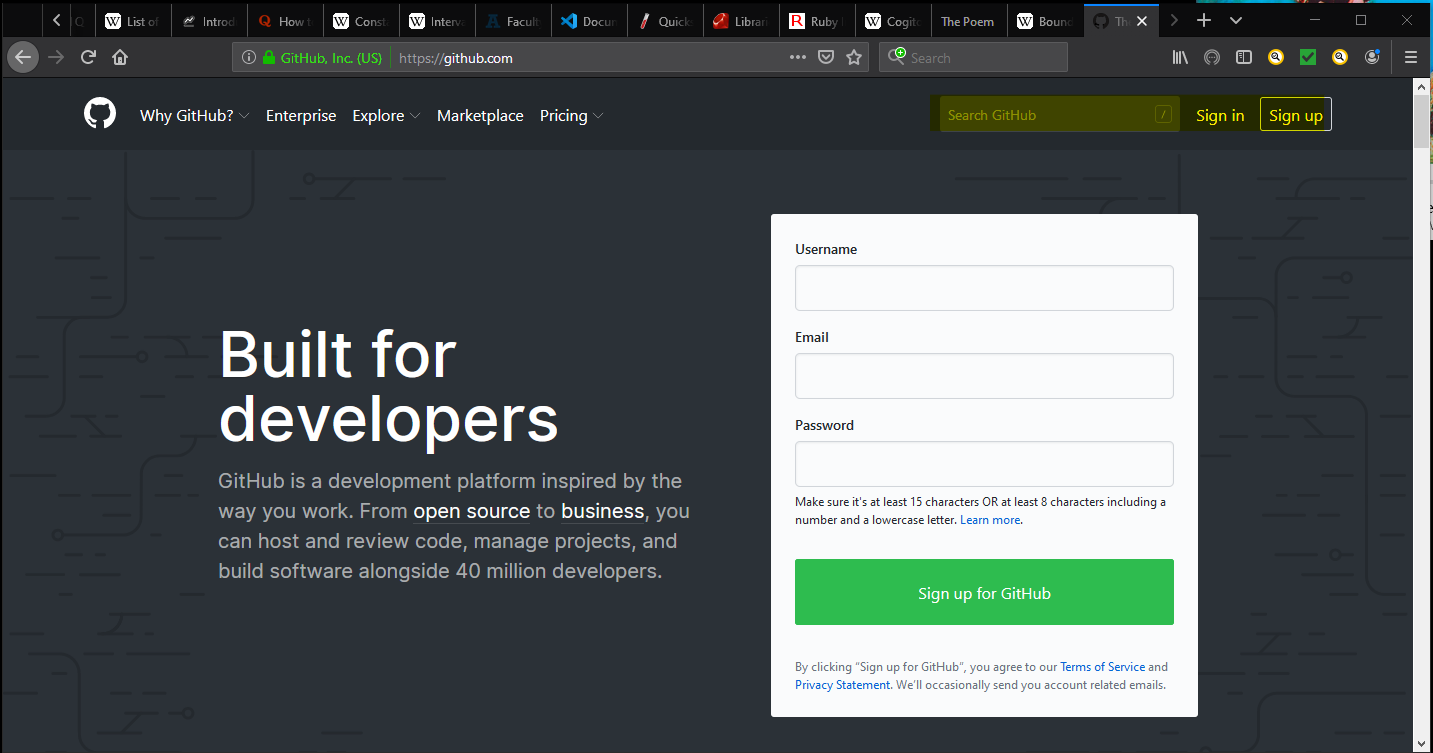
\includegraphics{../images/github_01.png}
\caption{{Screenshot} taken using {\bf Snip \& Sketch}. This is an app on
         my Windows 10 box}
\end{figure}
\eject
%%%%%%%%%%%%%%%%%%%%%%%%%%%%%%%%%%%%%%%%%%%%%%%%%%%%%%%%%%%%%%%%%%%%%%%%%%%%%%%%
%%%%%%%%%%%%%%%%%%%%%%%%%%%%%%%%%%%%%%%%%%%%%%%%%%%%%%%%%%%%%%%%%%%%%%%%%%%%%%%%
\vskip0.1in\hrule\vskip0.1in
\noindent
{\bf Homework Repository for Math 4610: Login to Your Account.} 
\vskip0.1in\hrule\vskip0.1in
Use the popup to login to Github with your user name and password.
\vfill
\begin{figure}[h]
\centering
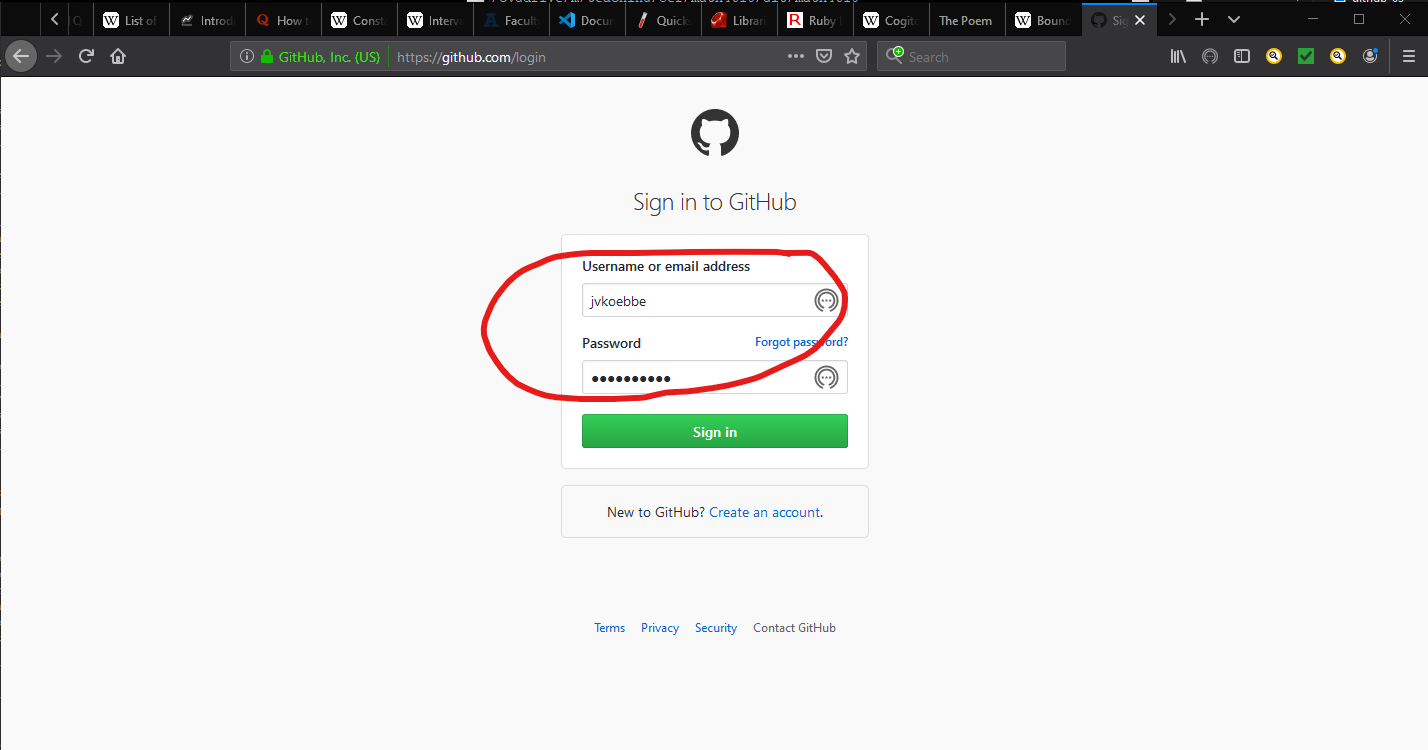
\includegraphics{../images/github_02.png}
\caption{{Screenshot} taken using {\bf Snip \& Sketch}. This is an app on
         my Windows 10 box}
\end{figure}
\eject
%%%%%%%%%%%%%%%%%%%%%%%%%%%%%%%%%%%%%%%%%%%%%%%%%%%%%%%%%%%%%%%%%%%%%%%%%%%%%%%%
%%%%%%%%%%%%%%%%%%%%%%%%%%%%%%%%%%%%%%%%%%%%%%%%%%%%%%%%%%%%%%%%%%%%%%%%%%%%%%%%
\vskip0.1in\hrule\vskip0.1in
\noindent
{\bf Homework Repository for Math 4610: Starting Point for Working on a
Repostiroy.} 
\vskip0.1in\hrule\vskip0.1in
Once the following pops up, we can navigate in amongst the repositories if you
have more than one. In any case, you should have a repository named
\begin{verbatim}

    math4610

\end{verbatim}
Click on this repository to start creating files and the like. Once the
repository is created, students can click on the name to work on the repository
or use files in the repository.
\vfill
\begin{figure}[h]
\centering
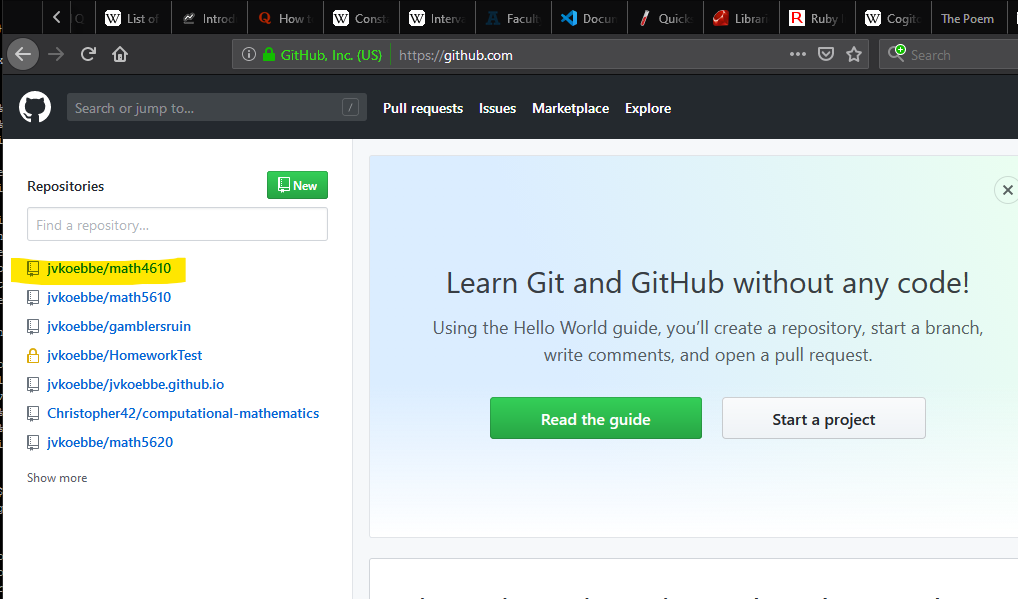
\includegraphics{../images/github_03.png}
\caption{{Screenshot} taken using {\bf Snip \& Sketch}. This is an app on
         my Windows 10 box}
\end{figure}
\eject
%%%%%%%%%%%%%%%%%%%%%%%%%%%%%%%%%%%%%%%%%%%%%%%%%%%%%%%%%%%%%%%%%%%%%%%%%%%%%%%%
%%%%%%%%%%%%%%%%%%%%%%%%%%%%%%%%%%%%%%%%%%%%%%%%%%%%%%%%%%%%%%%%%%%%%%%%%%%%%%%%
To start putting together the repository for submitting task solutions, students
can create a new file by clicking on the button as shown below. In particular,
students should create the table of contents file for the task sheets.
\vfill
\begin{figure}[h]
\centering
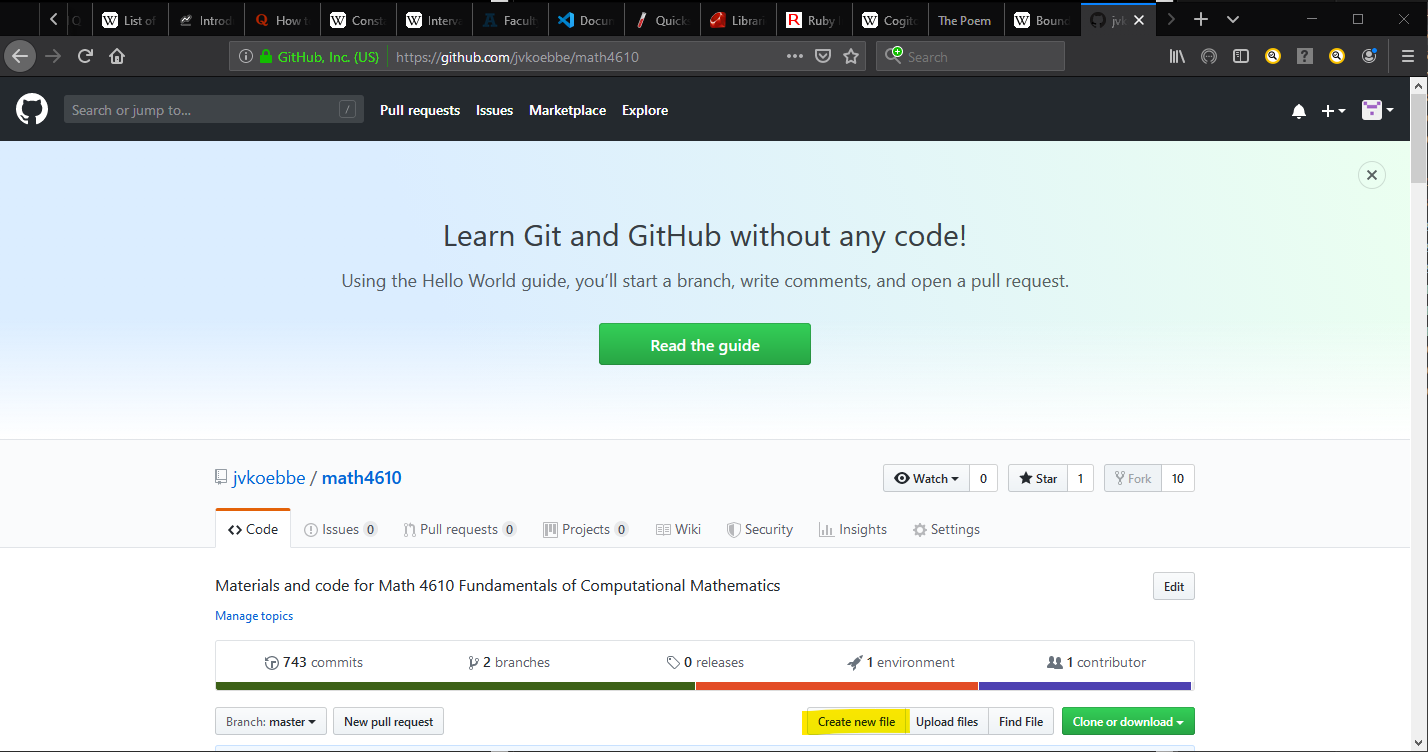
\includegraphics{../images/github_04.png}
\caption{{Screenshot} taken using {\bf Snip \& Sketch}. This is an app on
         my Windows 10 box}
\end{figure}
\eject
%%%%%%%%%%%%%%%%%%%%%%%%%%%%%%%%%%%%%%%%%%%%%%%%%%%%%%%%%%%%%%%%%%%%%%%%%%%%%%%%
%%%%%%%%%%%%%%%%%%%%%%%%%%%%%%%%%%%%%%%%%%%%%%%%%%%%%%%%%%%%%%%%%%%%%%%%%%%%%%%%
In the following figure, two things should be noted. The first is the name of
the file
\begin{verbatim}

    hw_toc.md

\end{verbatim}
Note that the extension, \lq\lq .md\rq\rq\ indicates to a browser tha this is a
MarkDown file. We will spend more time on using MarkDown in this and other
lectures in the course. The second piece of the puzzle is the circled region
where you can type in lines that will be used in the file. All you need to do is
click to the right of the numbered line and start typing.
\vfill
\begin{figure}[h]
\centering
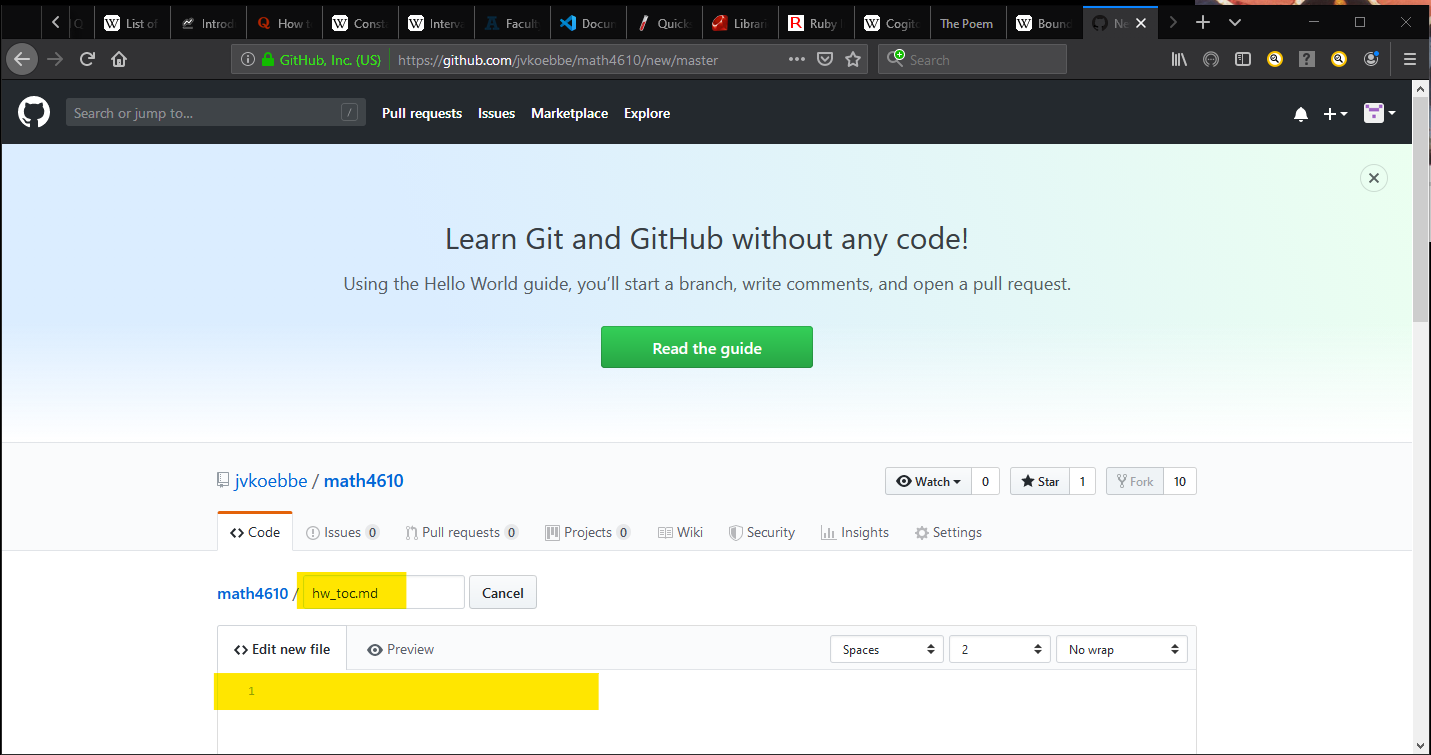
\includegraphics{../images/github_05.png}
\caption{{Screenshot} taken using {\bf Snip \& Sketch}. This is an app on
         my Windows 10 box}
\end{figure}
\eject
%%%%%%%%%%%%%%%%%%%%%%%%%%%%%%%%%%%%%%%%%%%%%%%%%%%%%%%%%%%%%%%%%%%%%%%%%%%%%%%%
%%%%%%%%%%%%%%%%%%%%%%%%%%%%%%%%%%%%%%%%%%%%%%%%%%%%%%%%%%%%%%%%%%%%%%%%%%%%%%%%
To give an idea of how to use MarkDown to set up a table of contents. Each of
the lines serve a function in the table of contents.
\begin{verbatim}

    # Math 4610 Homework Solutions

\end{verbatim}
This line is a header line due to the pound sign. The second nonblank line is a
header line with a smaller font size. Note that these lines are short hand in
HTML for <h1> and <h2>. The next two lines provide links to other files that
will contain your homework solutions. Note that the asterisk preceding the text
in these lines indicates a bullet should be placed in front of the text. There
are tasks in the homework that will walk you through at least some subset of
MarkDown syntax.
\vfill
\begin{figure}[h]
\centering
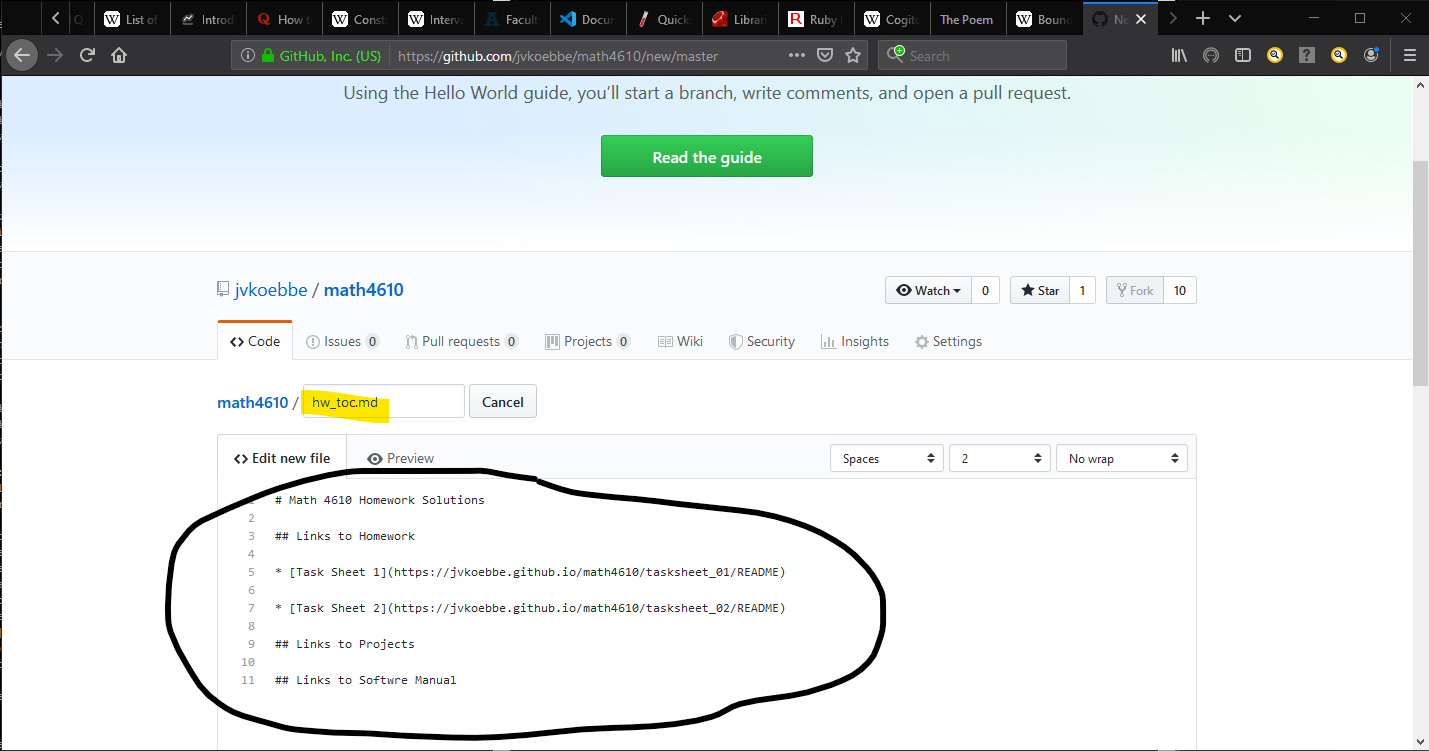
\includegraphics{../images/github_06.png}
\caption{{Screenshot} taken using {\bf Snip \& Sketch}. This is an app on
         my Windows 10 box}
\end{figure}
\eject
%%%%%%%%%%%%%%%%%%%%%%%%%%%%%%%%%%%%%%%%%%%%%%%%%%%%%%%%%%%%%%%%%%%%%%%%%%%%%%%%
%%%%%%%%%%%%%%%%%%%%%%%%%%%%%%%%%%%%%%%%%%%%%%%%%%%%%%%%%%%%%%%%%%%%%%%%%%%%%%%%
Version Control Systems (VCS) like git do not make changes to a repository 
unless a commit has been made. If you scroll down to the bottom of the webpage
there are a couple of boxes and buttons to consider. The textboxes allow the
user to enter comments about the changes being made to the repository. It is
strongly recommended that students add comments about the changes being made.
Finally, the is a button that will seal the deal on the modifications. To
push the changes, click on the
\begin{verbatim}

    Commit new file

\end{verbatim}
button. If you do not want to keep the changes, click on the
\begin{verbatim}

    Cancel

\end{verbatim}
If you cancel the changes, a popup will appear that will allow you to reconsider
the choice. So, click on the commit button.
\vfill
\begin{figure}[h]
\centering
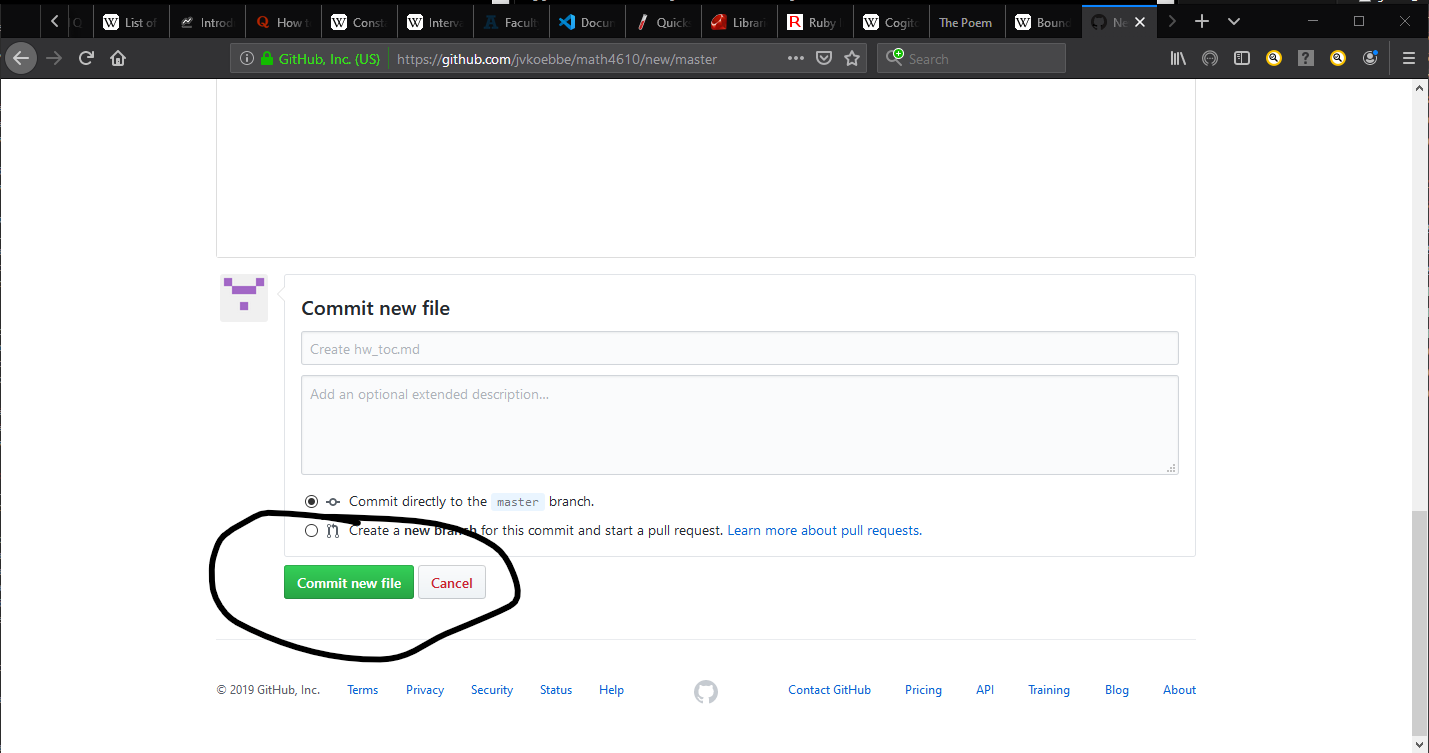
\includegraphics{../images/github_07.png}
\caption{{Screenshot} taken using {\bf Snip \& Sketch}. This is an app on
         my Windows 10 box}
\end{figure}
\eject
%%%%%%%%%%%%%%%%%%%%%%%%%%%%%%%%%%%%%%%%%%%%%%%%%%%%%%%%%%%%%%%%%%%%%%%%%%%%%%%%
%%%%%%%%%%%%%%%%%%%%%%%%%%%%%%%%%%%%%%%%%%%%%%%%%%%%%%%%%%%%%%%%%%%%%%%%%%%%%%%%
There are a couple of ways to create folders in a repository. One way is to go
back into the editor funcion on Github and modify the name of an existing file.
For this part of the lecture, a different repository will be used. Students
should use their math4610 repository to follow along with this example. To
start the process, create a file
\begin{verbatim}

    harmless.md

\end{verbatim}
You can include some text and then commit the change as shown above.
\vfill
\begin{figure}[h]
\centering
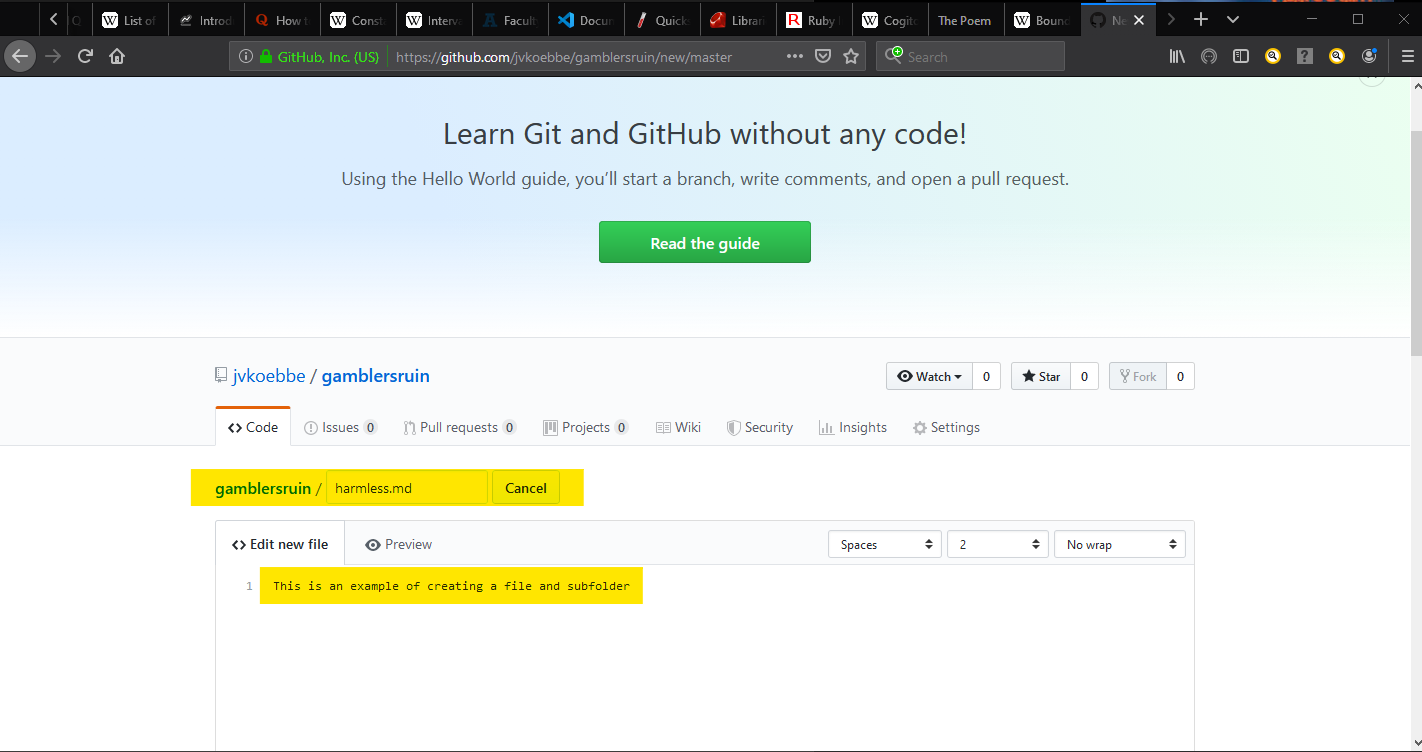
\includegraphics{../images/github_08.png}
\caption{{Screenshot} taken using {\bf Snip \& Sketch}. This is an app on
         my Windows 10 box}
\end{figure}
\eject
%%%%%%%%%%%%%%%%%%%%%%%%%%%%%%%%%%%%%%%%%%%%%%%%%%%%%%%%%%%%%%%%%%%%%%%%%%%%%%%%
%%%%%%%%%%%%%%%%%%%%%%%%%%%%%%%%%%%%%%%%%%%%%%%%%%%%%%%%%%%%%%%%%%%%%%%%%%%%%%%%
Next, click on the repositry name at the top of the webpage. Students should see
the file name
\begin{verbatim}

    harmless.md

\end{verbatim}
in the list of files. Click on the filename in the list to show the contents of
the file.
\vfill
\begin{figure}[h]
\centering
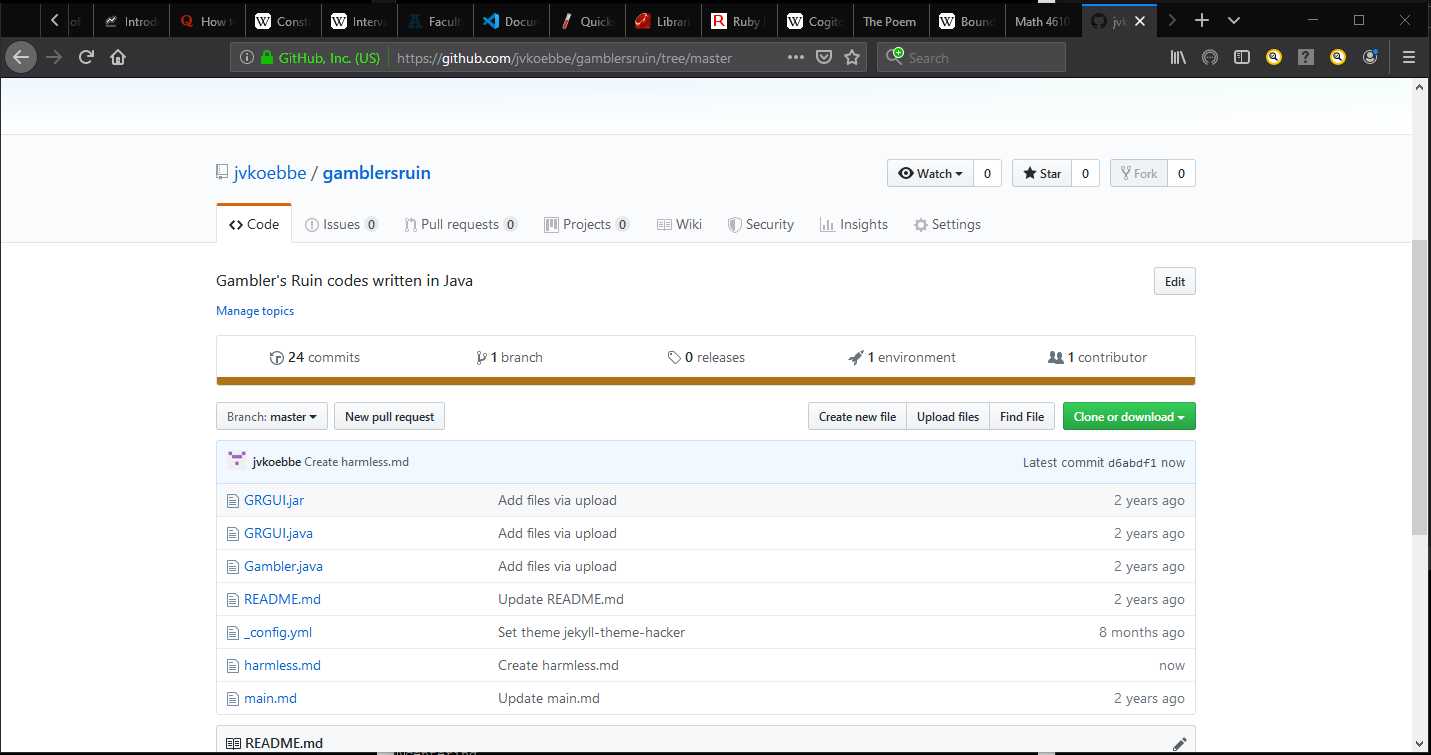
\includegraphics{../images/github_09.png}
\caption{{Screenshot} taken using {\bf Snip \& Sketch}. This is an app on
         my Windows 10 box}
\end{figure}
\eject
%%%%%%%%%%%%%%%%%%%%%%%%%%%%%%%%%%%%%%%%%%%%%%%%%%%%%%%%%%%%%%%%%%%%%%%%%%%%%%%%
%%%%%%%%%%%%%%%%%%%%%%%%%%%%%%%%%%%%%%%%%%%%%%%%%%%%%%%%%%%%%%%%%%%%%%%%%%%%%%%%
Once the file contents are displayed, we can edut the 
\vfill
\begin{figure}[h]
\centering
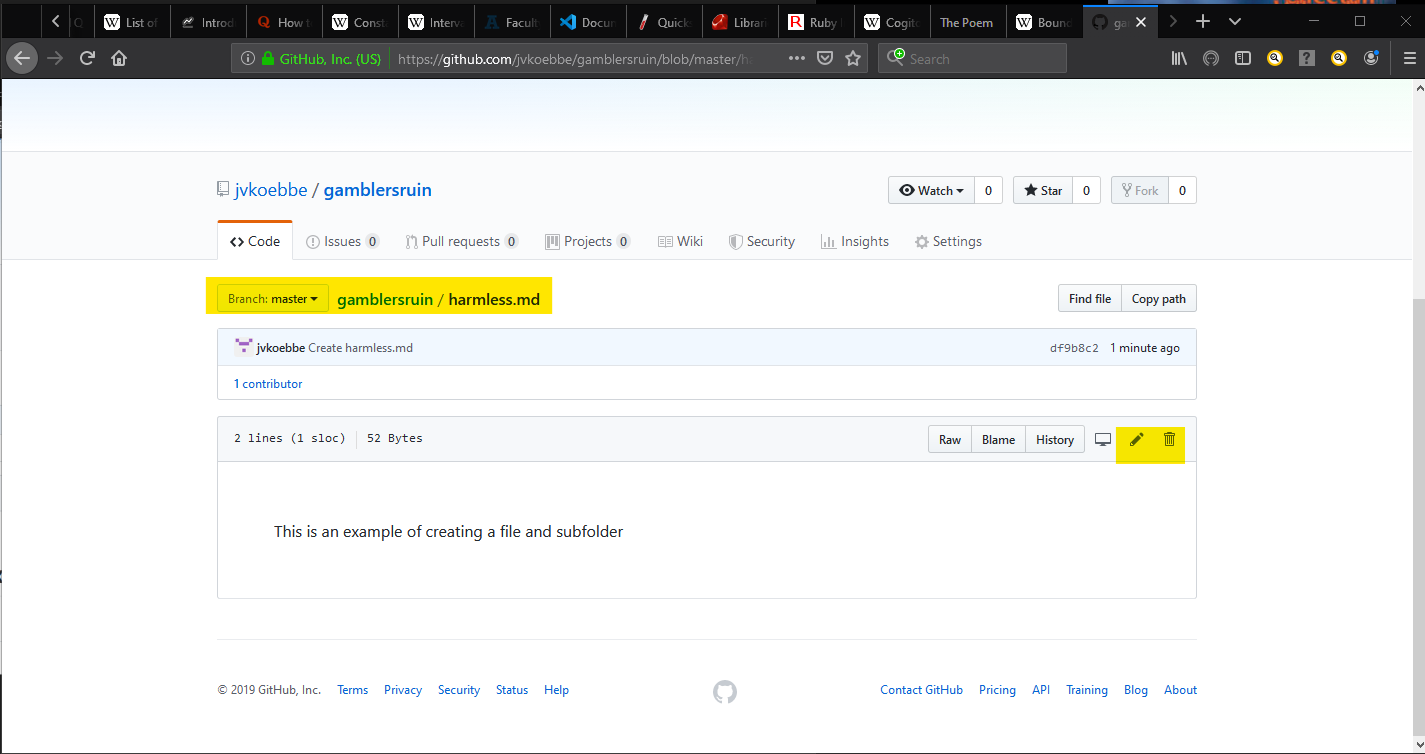
\includegraphics{../images/github_10.png}
\caption{{Screenshot} taken using {\bf Snip \& Sketch}. This is an app on
         my Windows 10 box}
\end{figure}
\eject
%%%%%%%%%%%%%%%%%%%%%%%%%%%%%%%%%%%%%%%%%%%%%%%%%%%%%%%%%%%%%%%%%%%%%%%%%%%%%%%%
%%%%%%%%%%%%%%%%%%%%%%%%%%%%%%%%%%%%%%%%%%%%%%%%%%%%%%%%%%%%%%%%%%%%%%%%%%%%%%%%
button that will create a new file.
\vfill
\begin{figure}[h]
\centering
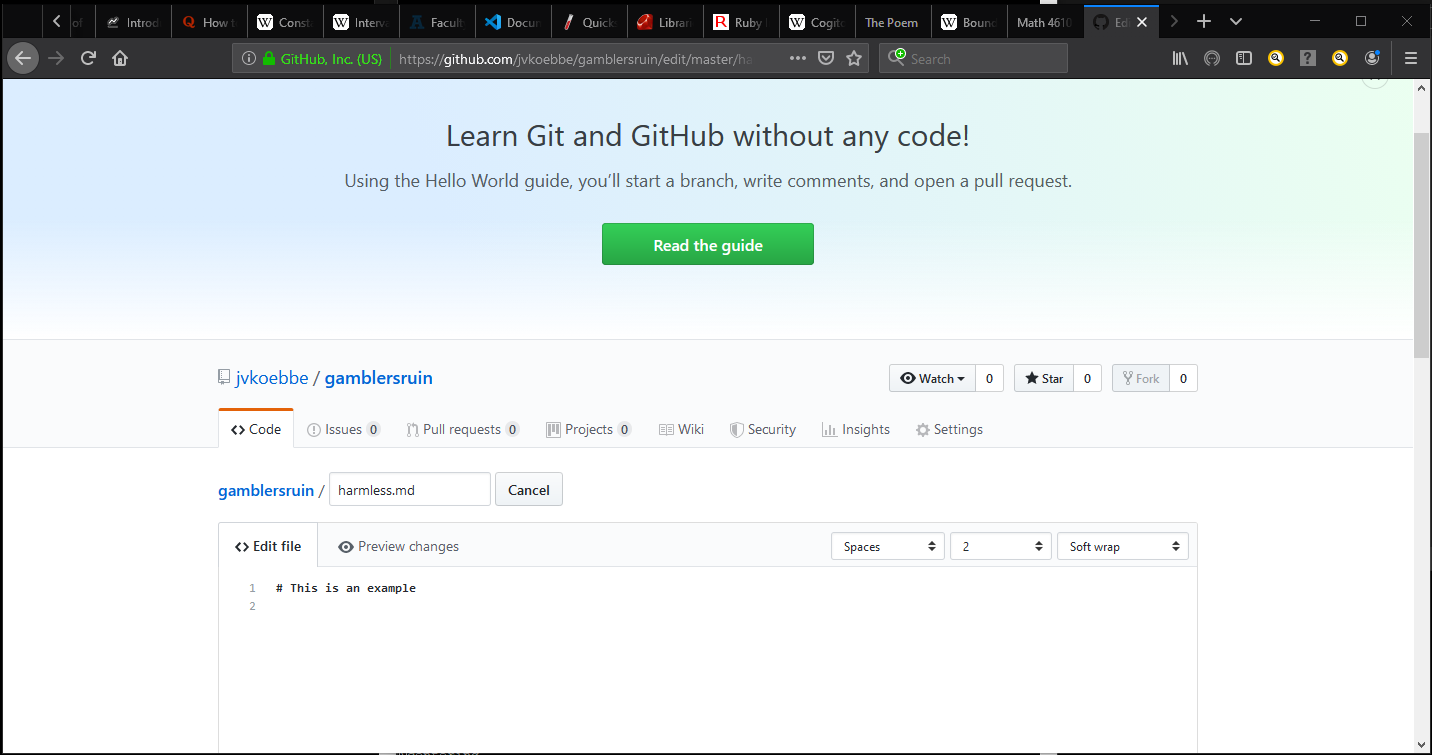
\includegraphics{../images/github_11.png}
\caption{{Screenshot} taken using {\bf Snip \& Sketch}. This is an app on
         my Windows 10 box}
\end{figure}
\eject
%%%%%%%%%%%%%%%%%%%%%%%%%%%%%%%%%%%%%%%%%%%%%%%%%%%%%%%%%%%%%%%%%%%%%%%%%%%%%%%%
%%%%%%%%%%%%%%%%%%%%%%%%%%%%%%%%%%%%%%%%%%%%%%%%%%%%%%%%%%%%%%%%%%%%%%%%%%%%%%%%
button that will create a new file.
\vfill
\begin{figure}[h]
\centering
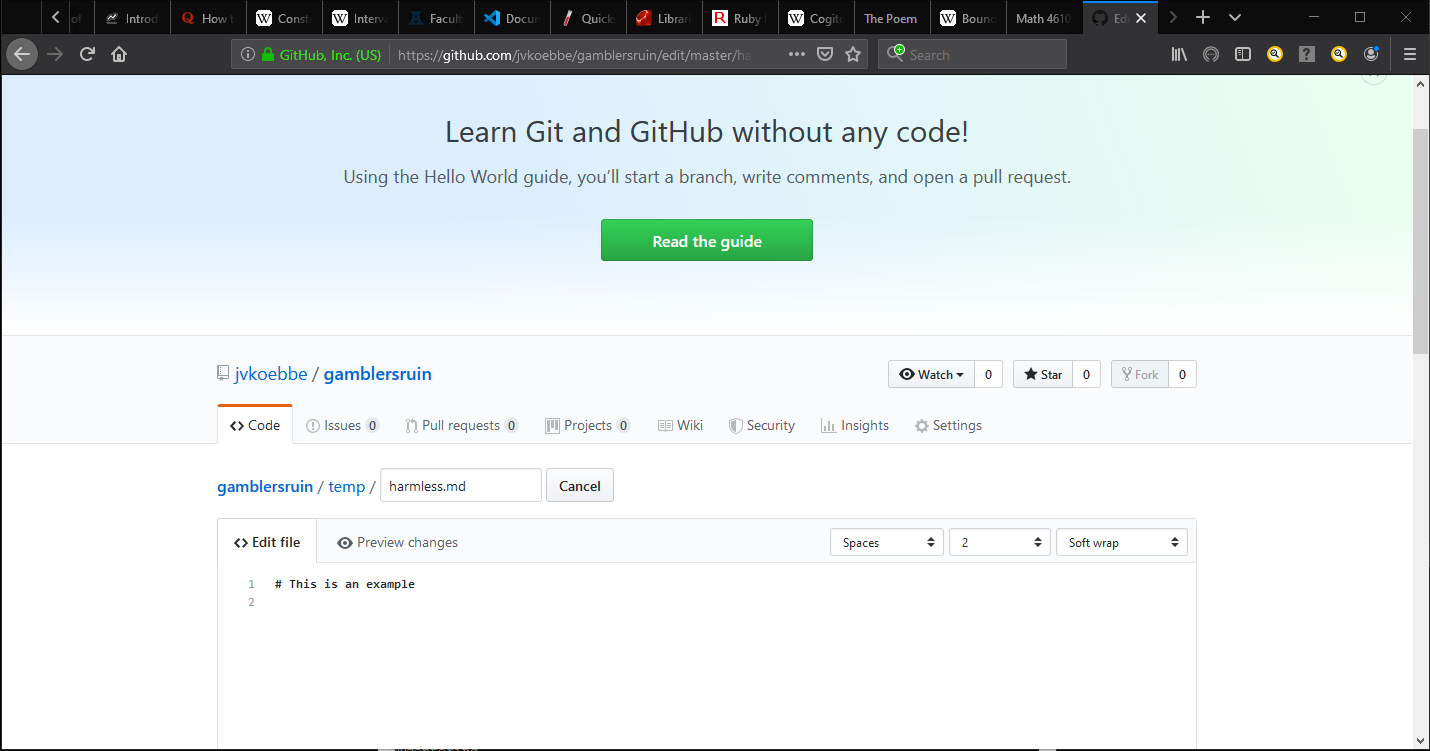
\includegraphics{../images/github_12.png}
\caption{{Screenshot} taken using {\bf Snip \& Sketch}. This is an app on
         my Windows 10 box}
\end{figure}
\eject
%%%%%%%%%%%%%%%%%%%%%%%%%%%%%%%%%%%%%%%%%%%%%%%%%%%%%%%%%%%%%%%%%%%%%%%%%%%%%%%%
%%%%%%%%%%%%%%%%%%%%%%%%%%%%%%%%%%%%%%%%%%%%%%%%%%%%%%%%%%%%%%%%%%%%%%%%%%%%%%%%
button that will create a new file.
\vfill
\begin{figure}[h]
\centering
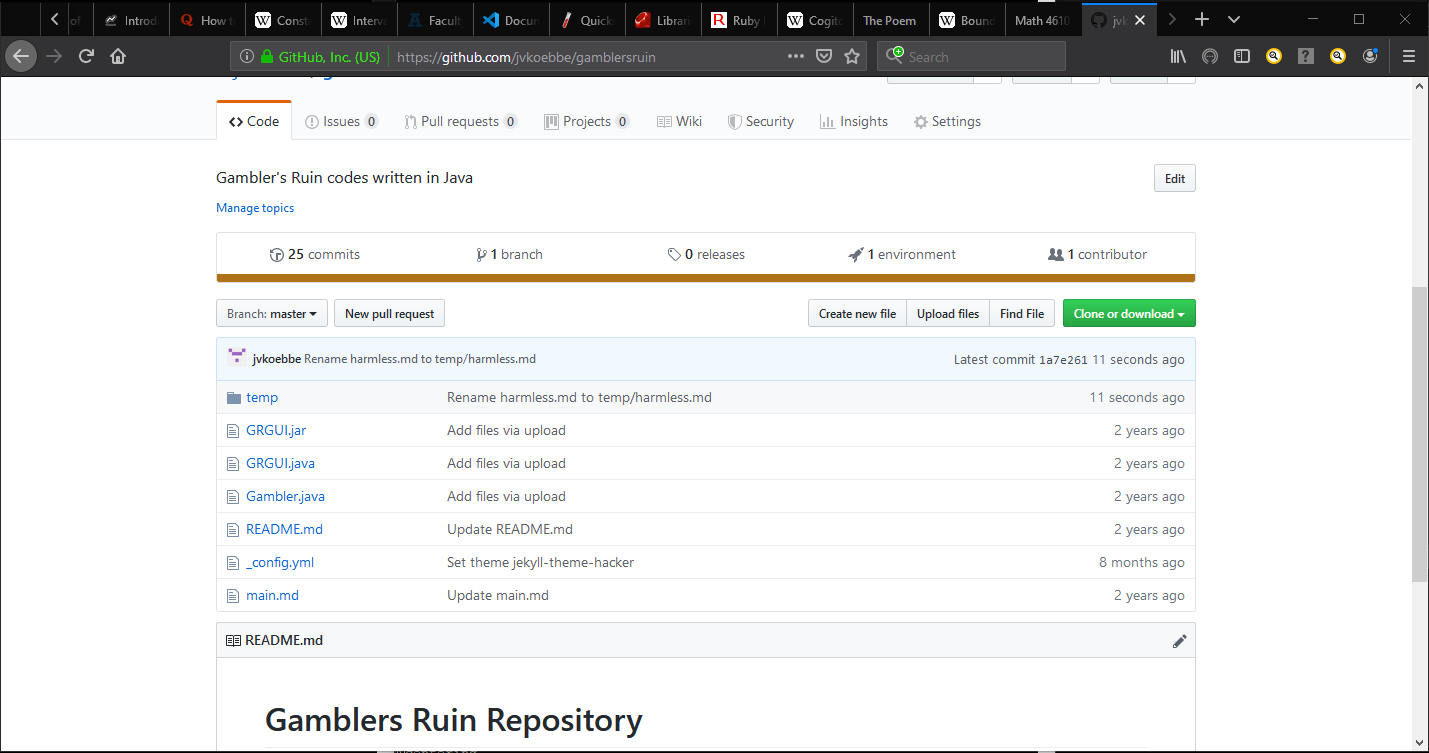
\includegraphics{../images/github_13.png}
\caption{{Screenshot} taken using {\bf Snip \& Sketch}. This is an app on
         my Windows 10 box}
\end{figure}
\eject
%%%%%%%%%%%%%%%%%%%%%%%%%%%%%%%%%%%%%%%%%%%%%%%%%%%%%%%%%%%%%%%%%%%%%%%%%%%%%%%%
%%%%%%%%%%%%%%%%%%%%%%%%%%%%%%%%%%%%%%%%%%%%%%%%%%%%%%%%%%%%%%%%%%%%%%%%%%%%%%%%
\end{document}
